\chapter{Accumulation of a Food Image Dataset}
\lhead{\emph{Accumulation of a Food Image Dataset}}

Before starting to experiment with machine learning algorithms for food classification, a dataset of food images needed to be created. In this chapter, reasons, why the dataset is required, are going to be explained and a process of accumulating the dataset is going to be described.

\section{The Requirements for the Food Image Dataset}
 The dataset was needed because classification algorithms use the dataset to learn a classification model from it. The most important requirements to the dataset were:

\begin{enumerate}
  \item The images of the dataset should be taken under a real life conditions.
  \item There should be enough pictures in the dataset to learn the model for every machine learning algorithm that is going to be tried.
  \item Variance of food images of the same class should be high. 
\end{enumerate}

Real life condition pictures were needed, because of the intention to create a model that could classify pictures of food taken by people using cameras of mobile phones, it was critical that food images in the dataset could not be created in lab conditions. People use different angles and distance for taking pictures. The light conditions in images often vary greatly too. It was crucial to represent these conditions in the food image dataset.

The dataset also needed to have many images belonging to each class. Having a lot of training samples is the best way to make sure that the model learned is generalised enough to perform well on a test dataset. Simple models trained on a lot of data perform better than more elaborate models based on less data \citep{unreasonable}.Because of that, it was decided that around 1,000 training images are needed for each class of food in the dataset. 

Finally, an intraclass class variance of pictures in the training dataset should also be high. The problem of datasets with little variance can be illustrated with a dataset of tree images containing only pictures of trees with green leaves.The model learned by a classifier from this dataset will always classify a tree with orange leaves or a tree without leaves as a not tree. Therefore, a food dataset should also include a different kind of images for the same class e.g. pizza with cheese, pepperoni pizza, a slice of pizza, etc. 

Accumulation of the dataset that satisfies these requirements was a challenging task. It would take a long time to take enough photos of meals for creating a big enough dataset. Also, a dataset containing images taken by only one or a few persons would not have enough variance. Because of that, possibilities to download food images from the Internet had to be explored.


It was observed that there are a lot of food images hosted on a photo sharing service flickr.com. After reading that Flickr has a Python API that could be used for searching for images according to their tags or titles and then downloading these images resized to the specified resolution, it was decided to write a Python script using this API. After downloading the images with a tag ``Fish and Chips",  it was realized that there were a lot of images that contained this tag but were not actual food pictures e.g. \autoref{fig:fish}. Because of the time it takes to review every image downloaded and delete pictures that do not represent the class, it was decided to try to find a public food image dataset with images that were already classified.  


\begin{figure}[ht]
\centering
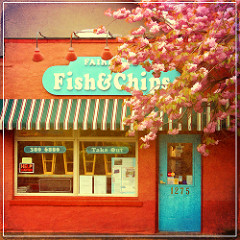
\includegraphics[width=2cm]{Figures/c3/flick.jpg}
\caption{Example of an image with a fish and chips tag, downloaded using the Flickr API}
\label{fig:fish}
\end{figure}


It was found that ImageNet Classification challenge, that was briefly described in \autoref{sec:intro}  includes many categories of food pictures. The only problem was that the number of images in different classes varies widely. Some classes like pizza have around 1300 pictures while other classes like salmon loaf have only 360 pictures. This problem was only discovered later when it was observed that when training K-NN classifier chicken with rice class, which had around two times less training examples than other classes was selected notably less as a target class of testing images. Because of that four image categories which all have around 1300 of images was chosen from the image Net data set. These four classes were fish and chips, pizza, salad and vanilla ice-cream. 

Four classes of images were picked because the data set required to be small enough to be trained on a laptop computer.  Using food of four classes allows machine learning algorithms to be trained faster. That means that various configurations of algorithms can be explored without having to wait very long to see the final result. Also, it was considered that after investigating machine learning algorithms on four-class classification problem, it would be a relatively easy task to retrain the algorithm using different data set containing either more classes of food images or a different set of classes.

\section {Downloading the Dataset}
Since ImageNet publicly only provides links to the original hosts of image files,  a Python Script was written to read links from text files, download the images from these links and save them to disk.  The first problem that was faced after downloading the images was that many pictures were either corrupted or were template images provided by hosting sites that said that the photo was no longer available. The script was modified to solve this problem by aborting the download and moving on to a next image if a server returned a HTTP redirect code. This code modification solved the problem of wrong images appearing in the downloaded data set. However, because many images were no longer available to download from the hosting sites, the data set become much smaller than originally planned.  

To overcome this problem, permission to access the original ImageNet download files was requested. After agreeing to use the data set only for non-commercial research and educational purposes, the permission to download the database was granted. It allowed accessing the original data set with all images included. The original archives were downloaded using a python method described in the following section.  Each class of downloaded images contained approximately 1,300 pictures.

\section {Image Preprocessing}
Python class named Data was created to handle a creation of the image data set. The class is very flexible and allows images to be loaded using various ways. The constructor of the class takes one argument: the relative path to the folder, where the data is located. Then, images can be loaded from a pickle file located in /pickle folder or can be read directly from a /images folder. It is recommended to save the files to a pickle file after reading the files from a /images folder for the first time. A pickle is a binary file representing a Python object. Reading the dataset from a pickle takes much less time than reading images one by one because Python only needs to read one file compared to thousands of files while loading images. To be loaded correctly, the pickle should be structured as a list of labels of every picture, followed by a list of images. Method try\_download\_images is provided in this class to download the data set from ImageNet. It takes two arguments: username and ImageNet access key, downloads the archive of images for each image class. The method named extract can be used to extract downloaded .tar archive files into the pictures folder. Before extracting each archive, it checks if files already exist and if that is the case extraction is aborted. Method resize\_image can be used for resizing images in the dataset. It takes a list with height and width of requested image size and resizes the images.  Finally, train\_test\_split method can be used to shuffle the data and split it into training and testing datasets. It takes an optional argument- a fraction that shows a percentage of data to be used for testing the classifier.

\section{Summary}
In this chapter, the requirements for the dataset were defined. The most important rule for the image dataset was to have many pictures that were taken under real life conditions in each class.  Because of this requirement, it was decided to download food images from the ImageNet. To reducing the complexity, only four food classes were selected: fish and chips, pizza, salad and vanilla ice-cream. Finally, the dataset was split into training and testing datasets.  In the following chapter, machine learning algorithms will be used to train the food classification models.